% Modified 31 Oct 2005:  Conditioning fallacy alluded to.
% This chapter has been modified on 6-4-05.
% There are two \choice
\pagestyle{headings}
\setcounter{chapter}{0}
\chapter{Foundations of Probability} \label{chp 1}
\thispagestyle{fancy}
\setcounter{page}{1}

\subsection*{Introduction: The Monty Hall Problem}\index{Monty Hall Problem}
In a certain popular game show, the contestant is offered a chance to win a car. She must choose one of three doors; behind one of the doors is a car, and behind the other two are goats. She has no evidence to help her determine which prize is behind which door, so assuming no collusion between the contestant and the game show producers, she has no reason to prefer any one door to any other.
\par
After the contestant has made her choice, the host then opens a door. The host will never open the door that the contestant has chosen, and will always open a door with a goat behind it. This is possible since there are two doors with goats behind them. At this point, the host offers the contestant a chance to switch her choice from the door she initially chose to the other remaining unopened door. 
\par
How does the decision to switch doors affect her chance of winning the car?
\begin{itmize}
\item Switching \emx{increases} her chance of winning from $1/3$ to $1/2$.
\item Switching \emx{increases} her chance of winning from $1/3$ to $2/3$.
\item Switching \emx{decreases} her chance of winning from $1/3$ to $1/6$.
\item Her chance of winning is $1/3$ regardless of whether she switches or not.
\item Her chance of winning is $1/2$ regardless of whether she switches or not.
\end{itmize}
\par
This is a classic puzzle posed in a letter to the editors of American Statistician \cite{MontyHallOriginal}, later popularized in the `Ask Marilyn' column of Parade magazine \cite{vosSavant}. Debate over the correctness of the (correct) answer given there has raged ever since.
\par
We have very strong intuitions about probability, which can sometimes be an aid and sometimes be a hindrance. In order to resolve the problem above in a manner which will be clear and convincing, even to individuals whose intuitions lead them to different conclusions, we need to establish some notation and fundamental laws we all agree on.
\newpage

\section{Sample Spaces \& Events} \label{sec 1.1}

Suppose that the outcome of some experiment is uncertain, but we can write down the set of all possible outcomes in advance. This set of possible outcomes is known as a \emx{sample space}, and is the most basic object in the theory of probability. Precisely specifying a sample space will clarify the context of a problem and eliminate many potential sources of confusion.

\begin{definition} The set of possible outcomes of an experiment is known as a sample space\index{Sample Space}, and typically denoted $\Omega$.
\end{definition}
\begin{examp}Consider a single roll of a single die. In this experiment, there are six possible outcomes, corresponding to the six distinct faces of the die. Thus, we take $\Omega = \{1,2,3,4,5,6\}$.
\end{examp}
\begin{examp}\label{breakingstrength}Consider measuring the breaking strength (in Newtons) of a plank of wood. If we have no information about the size or shape of the plank, or about the precision with which the breaking strength will be measured, we should allow any positive value. Thus, $\Omega = \{x \in \mathbb{R} \, | \, x \geq 0\}$.\end{examp}
\begin{examp}Suppose that a coin is flipped, and then a marble is drawn from an urn which contains black, white, and grey marbles. In this scenario, we could take $\Omega = \{HB,HW,HG,TB,TW,TG\}$, using $HB$ to represent flipping a head and drawing a black marble, $HW$ to represent flipping a head and drawing a white marble, and so on. \end{examp}
\begin{examp}\label{FlipUntilTail}Suppose you play a game where a coin is flipped repeatedly until the first tail appears. We could take $\Omega = \{T, HT, HHT, HHHT, HHHHT, \, ...\, \}$. \end{examp}
\par
If the outcomes in a sample space can be listed (whether that list is finite or infinite) it is \emx{discrete}\index{Sample Space!discrete}, and if the set of all outcomes forms a continuum, as in the case of Example \ref{breakingstrength}, then the sample space is \emx{continuous}\index{Sample Space!continuous}.
\par
The choice of sample space depends on the experiment and on what question we as experimenters are trying to answer. If we roll a pair of dice, we might use the sample space $\Omega = \{2,3,4,\,...\,,11,12\}$ to count the sum of the two resulting values, or $\Omega = \{(1,1),(1,2),(2,1),(2,2),\,...\,,(5,6),(6,5),(6,6)\}$ to distinguish the dice and represent the values on each, so situations such as rolling doubles can be noted.
\par
Another advantage of the larger sample space is that each of the outcomes is \emx{equally likely}. Imagine one die is red and the other is blue (changing the colours of the dice certainly won't influence the results of the experiment). If neither die has any bias, then when the pair is rolled, each die is equally likely to land with any of its faces up. The red die showing 2 and blue showing 5 is as likely as the red die showing 6 and blue showing 6, and so on. Each ordered pair of outcomes $(m,n)$ for $1 \leq m \leq 6$ and $1 \leq n \leq 6$ is as likely as any other.
\par
If we write the number showing on the red die across the top row, the number showing on the blue die down the left column, and the sum of the two results in a table, we obtain the following.
{\small
\begin{center}
\begin{tabular}{c|cccccc}
$_{B} \setminus ^R$ & 1 & 2 & 3 & 4 & 5 & 6 \\
\hline
1 & 2 & 3 & 4 & 5 & 6 & 7 \\
2 & 3 & 4 & 5 & 6 & 7 & 8 \\
3 & 4 & 5 & 6 & 7 & 8 & 9 \\
4 & 5 & 6 & 7 & 8 & 9 & $\!$10 \\
5 & 6 & 7 & 8 & 9 & $\!$10 & $\!$11 \\
6 & 7 & 8 & 9 & $\!$10 & $\!$11 & $\!$12 \\
\end{tabular}
\end{center}
}
Note that outcomes in the sample space $\Omega = \{2,3,4,\,...\,,11,12\}$ are \emx{not equally likely}. There are six ordered pairs $(1,6)$, $(2,5)$, $(3,4)$, $(4,3)$, $(5,2)$, and $(6,1)$ which yield a sum of seven, while only the single pair $(1,1)$ gives a sum of two.
\subsection*{Events in a Sample Space}
\begin{definition}
Events\index{Event} are certain subsets of a sample space in which we might be interested, and are denoted by capital letters. We can describe an event using words or with more formal set notation.
\end{definition}
\begin{examp}
Suppose we roll a single die. Let $\Omega = \{1,2,3,4,5,6\}$, let $A$ be the event `an even number is rolled' and let $B$ be the event `a number greater than four is rolled'. Then we can write $A = \{2,4,6\}$ and $B = \{5,6\}$.
\end{examp}
\begin{examp}\label{unitsquare}
Consider a point selected at random inside a square with corners at $(0,0)$, $(1,0)$, $(0,1)$, and $(1,1)$. Let $\Omega = \{(x,y) \, | \, 0 \leq x \leq 1$ and $0 \leq y \leq 1\}$, and let $T$ be the event `the point is in the top half of the square'. Then using set notation we would write $T = \{(x,y) \, | \, 0 \leq x \leq 1$ and $0.5 \leq y \leq 1\}$.
\end{examp}
\par
Given two events $A, B \subseteq \Omega$, we can use the usual set operations of \emx{intersection}\index{Intersection}, \emx{union}\index{Union}, and \emx{complement}\index{Complement} to form the events $A \cap B$ (both $A$ and $B$ occur), $A \cup B$ (at least one of $A$ and $B$ occurs), and $A^{c}$ ($A$ does not occur). Another useful operation is the \emx{set difference}\index{Events!difference of}\index{Difference}, which is denoted $A \backslash B$, and defined by $A \backslash B = A \cap B^{c}$.
\par
One can interpret $\cap$ as `and', $\cup$ as `or', and $^{c}$ as `not', but remember that $\cup$ refers to the \emx{inclusive or}, as in `to participate you must be older than 16 or have permission of a parent' (\emx{possibly both!}), not the \emx{exclusive or}, as in `the meal comes with a choice of soup or salad' (\emx{not both!}).
\par
\begin{center}
\begin{minipage}{1.6in}
\begin{center}
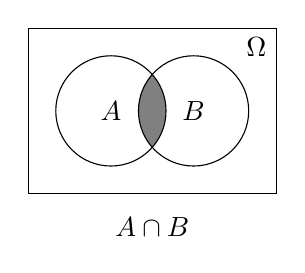
\begin{tikzpicture}[scale=0.7]
\draw (-1.5,-1.5) rectangle (3.0,1.5) node[below left]{$\Omega$};
\draw (1.6,-1.75) node[below left]{$A \cap B$};
\begin{scope}                       % start of clip scope
\clip (0,0) circle (1cm);
\fill[white] (0,0) circle (1cm);
\end{scope}                         % end of clip scope
\begin{scope}                       % start of clip scope
\clip (1.5,0) circle (1cm);
\fill[white] (1.5,0) circle (1cm);
\end{scope}                         % end of clip scope
\begin{scope}                       % start of clip scope
\clip (0,0) circle (1cm);
\fill[gray] (1.5,0) circle (1cm);
\end{scope}                         % end of clip scope
\draw (0,0) circle (1cm) node[] {$A$};
\draw (1.5,0) circle (1cm) node[] {$B$};
\end{tikzpicture}
\end{center}
\end{minipage}\begin{minipage}{1.6in}
\begin{center}
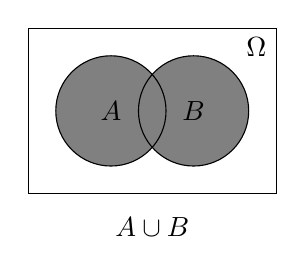
\begin{tikzpicture}[scale=0.7]
\draw (-1.5,-1.5) rectangle (3.0,1.5) node[below left]{$\Omega$};
\draw (1.6,-1.75) node[below left]{$A \cup B$};
\begin{scope}                       % start of clip scope
\clip (0,0) circle (1cm);
\fill[gray] (0,0) circle (1cm);
\end{scope}                         % end of clip scope
\begin{scope}                       % start of clip scope
\clip (1.5,0) circle (1cm);
\fill[gray] (1.5,0) circle (1cm);
\end{scope}                         % end of clip scope
\draw (0,0) circle (1cm) node[] {$A$};
\draw (1.5,0) circle (1cm) node[] {$B$};
\end{tikzpicture}
\end{center}
\end{minipage}
\end{center}

\begin{center}
\begin{minipage}{1.6in}
\begin{center}
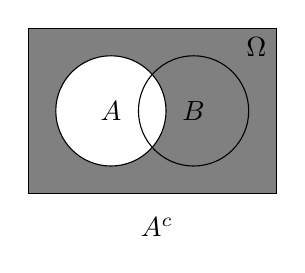
\begin{tikzpicture}[scale=0.7]
\begin{scope}                       % start of clip scope
\fill[gray] (-1.5,-1.5) rectangle (3.0,1.5);
\draw (1.3,-1.75) node[below left]{$A^c$};
\fill[white] (0,0) circle (1cm);
\end{scope}                         % end of clip scope
\draw (0,0) circle (1cm) node[] {$A$};
\draw (1.5,0) circle (1cm) node[] {$B$};
\draw (-1.5,-1.5) rectangle (3.0,1.5) node[below left]{$\Omega$};
\end{tikzpicture}
\end{center}
\end{minipage}\begin{minipage}{1.6in}
\begin{center}
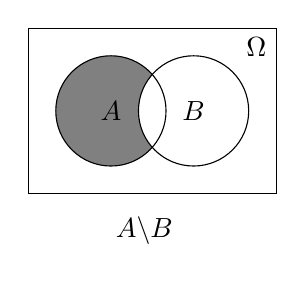
\begin{tikzpicture}[scale=0.7]
\begin{scope}                       % start of clip scope
\fill[gray] (0,0) circle (1cm);
\draw (1.3,-1.75) node[below left]{$A \backslash B$};
\fill[white] (1.5,0) circle (1cm);
\end{scope}                         % end of clip scope
\draw (0,0) circle (1cm) node[] {$A$};
\draw (1.5,0) circle (1cm) node[] {$B$};
\draw (-1.5,-1.5) rectangle (3.0,1.5) node[below left]{$\Omega$};
\end{tikzpicture}
\end{center}
\end{minipage}
\end{center}

\par
The set operations described above satisfy many laws, which together make up the \emx{algebra of sets}. Many of these laws are natural enough that there's likely no need for you to review them, for example $A \cup B = B \cup A$, or $(A^{c})^{c} = A$. However, it's probably worth reviewing \emx{DeMorgan's laws}\index{DeMorgan's Laws}. 
\eqnspar{(A \cap B)^{c} = A^{c} \cup B^{c} \text{ \ and \ } (A \cup B)^{c} = A^{c} \cap B^{c}}
\par 
We'll sometimes be dealing with long finite sequences of events $\{A_1, A_2, ...\,, A_n\}$ or infinite sequences $\{A_1, A_2, A_3, ...\}$ (also denoted $\{A_i\}_{i=1}^{\infty}$), so it's helpful to have some notation for abbreviating unions and intersections. We'll write large unions as below, and use similar notation for large intersections.
\eqns{\bigcup_{i=1}^{n} A_i = A_1 \cup A_2 \cup  ... \cup  A_n \text{\ \ and \ \ } \bigcup_{i=1}^{\infty} A_i = A_1 \cup  A_2 \cup  A_3 \cup  ... }
\par
\begin{examp}
In Example \ref{FlipUntilTail}, a coin is flipped until the first tail appears. If $A_k$ is the event `exactly $k$ heads are flipped', and $E$ is the event `a positive even number of heads are flipped', then $E = A_2 \cup A_4 \cup A_6 \cup ... = \bigcup_{i=1}^{\infty} A_{2i}$.
\end{examp}
\begin{examp}
Suppose that cards are drawn repeatedly from a deck until the first heart appears. Let $H_i$ denote the event `the i$^{th}$ card drawn is a heart', and let $T$ denote the event `at least ten cards are drawn before the first heart appears'. Then we have $T = {H_1}^c \cap {H_2}^c \cap ... \cap {H_{10}}^c = \bigcap_{i=1}^{10} {H_i}^c$. 
\end{examp}
\rmk DeMorgan's laws apply to sequences as well. This means we could rewrite the event $T$ in the example above as
\eqns{T = \bigcap_{i=1}^{10} {H_i}^c = {H_1}^c \cap {H_2}^c \cap ... \cap {H_{10}}^c = (H_1 \cup H_2 \cup ... \cup H_{10})^c = \left(\bigcup_{i=1}^{10} {H_i}\right)^{c}.}
\par
\noindent Note $\bigcup_{i=1}^{10}H_i$ is the event `at least one of the first ten cards drawn is a heart', so it's complement is `none of the first ten cards drawn is a heart', which is $T$.
\par
Let's return for a moment to rolling a pair of dice. Consider the events $N =$ `the sum of the two values showing is nine', $F =$ `one of the two dice shows a five', and $T = $ `one of the two dice shows a two'. Suppose that we roll the dice and $N$ occurs. Is it possible that $F$ also occurred? Yes. If one die shows a five and the other shows a four, then both events have occurred. What about $T$? If $N$ has occurred, it is possible that $T$ also occurred? This time the answer is no. If one of the dice shows two, the largest possible result would be eight. Thus, $N$ and $T$ cannot both occur when a pair of dice are rolled.
\begin{definition}\label{mutuallyexclusive}\index{Mutually Exclusive Events}\index{Events!mutually exclusive}
Two events $A$ and $B$ in a sample space $\Omega$ are mutually exclusive if $A \cap B = \emptyset$, that is, if there are no outcomes in $\Omega$ where both events occur.
\end{definition}
\begin{examp}
Consider an experiment where a coin is flipped, and then a die is rolled, and let $\Omega = \{H1,H2,H3,H4,H5,H6,T1,T2,T3,T4,T5,T6\}$. The events $H =$ `a head is flipped' and $E =$ `an even number is rolled' are not mutually exclusive, since $H \cap E = \{H2, H4, H6\}$.
\end{examp}
\begin{examp}
Suppose you're waiting for a bus, and you measure the number of seconds it takes for the bus to arrive. Let $E =$ `the bus arrives in under 3 minutes' and $F =$ `the bus takes more than 5 minutes to arrive'. Then $E$ and $F$ are mutually exclusive. Formally, let $\Omega = \{ x \in \mathbb{R} \, | \, x \geq 0\}$. In interval notation, we can write $E = [0,180)$ and $F = (300,\infty)$, then clearly $E \cap F = \emptyset$.
\end{examp}
\par
Extending the notion of mutually exclusive events given above in Definition \ref{mutuallyexclusive}, we call a finite or infinite sequence of events $\{A_1, A_2, A_3, ...\}$ mutually exclusive if for any pair of events $A_i$ and $A_j$ in the sequence, $A_i \cap A_j = \emptyset$.
\begin{examp}
In Example \ref{FlipUntilTail}, a coin is flipped until the first tail appears. If $A_k$ is the event `exactly $k$ heads are flipped', and $B_k$ is the event `at least $k$ heads are flipped', then $\{A_1, A_2, A_3, ...\}$ is a sequence of mutually exclusive events, while $\{B_1, B_2, B_3, ...\}$ is not since, for example, $B_2 \cap B_3 = \{HHHT, HHHHT, ...\}$.
\end{examp}

%\exercises
%\begin{LJSItem}

%\i\label{exer 1.1.1} In your pocket you have two nickels, three dimes, and a quarter. You reach into your pocket and remove two coins, one at a time.

%\begin{enumrate}
%\item Write a sample space which records the types of coins that were removed, and the order in which they were removed.
%\item Write a sample space which records only the amount of money removed.
%\end{enumrate}

%\i\label{exer 1.1.2} Write a sample space for the experiment of selecting a random point on the unit circle in $\mathbb{R}^2$.

%\i\label{exer 1.1.3} A certain email address receives a spam email from the same sender between 9:30 and 10:30 each day. Write a sample space for the time when the spam message arrives. (Careful, 9:65 is not a valid time, so you'll have to make a decision on how you record the arrival time)

%\i\label{exer 1.1.4} Alice and Bob each apply for several different jobs. Let $A =$ `Alice is hired' and $B =$ `Bob is hired'. Express the events below in terms of $A$ and $B$.

%\begin{enumrate}
%\item Alice is hired but not Bob.
%\item At least one of the two is hired.
%\item Exactly one of the two is hired.
%\end{enumrate}

%\i\label{exer 1.1.5} Colleges 1, 2, 3 and 4 are seeded into a basketball tournament in that order, so 1 will play 4 and 2 will play 3 in the first round. The winners will go on to play the final, and the losers will go on to play a relegation match. One possible outcome could be denoted 2413 (2 and 4 won their first games, then 2 beat 4 in the final and 1 beat 3 in the relegation match).

%\begin{enumrate}
%\item Write a sample space $\Omega$ listing all possible tournament outcomes, with each outcome denoted as above.
%\item Write the events $A =$ `1 wins the tournament' and $B =$ `2 plays in the final' as sets, then write $A \cap B$ as a set.
%\end{enumrate}

%\i\label{exer 1.1.6} Given any events $A$, $B$, and $C$, prove that $A \cap (B \cup C) = (A \cap B) \cup (A \cap C)$. (\emx{Hint}: There are many ways to do this, one is to simply draw a Venn digram for each side of the identity and observe that the shaded areas are the same)

%\i\label{exer 1.1.7} Prove DeMorgans's laws, $(A \cap B)^c = A^c \cup B^c$ and $(A \cup B)^c = A^c \cap B^c$.

%\i\label{exer 1.1.8} Suppose that a single card is drawn from a deck. Let $H =$ `the card is a heart' and $R =$ `the card is red'. Describe the events $A \cap R$, $A \cap R^c$, and $(A \cup R)^c$.

%\i\label{exer 1.1.9} Write an expression with indices which abbreviates each of the following.

%\begin{enumrate}
%\item $A_4 \cap A_5 \cap A_6 \cap ... \cap A_{21} \cap A_{22}$
%\item $A_1 \cup A_4 \cup A_7 \cup A_{10} \cup ... $
%\item $A_2 \cup A_4 \cup A_8 \cup ... \cup A_{128} \cup A_{256}$
%\end{enumrate}

%\i Let $\{A_i\}_{i=1}^{\infty}$ be an infinite sequence of events. Express the event `infinitely many of the $A_i$ occur' in terms of the events $A_i$. (\emx{Hint}: If finitely many occurred, then there must be a largest index $i$ for which $A_i$ occurred)

%\end{LJSItem}

\section{Axioms of Probability} \label{probaxiomssection}

The saying goes `you can't get something for nothing', and so it is in mathematics. However, you can get a lot for a little. The entirety of Euclidean plane geometry can be derived from a list of five simple statements. These foundational statements are known as axioms (greek for `that which is evident'). In probability theory, we can make do with only three axioms, proposed by Kolmogorov \cite{KolmogorovFoundations}\index{Kolmogorov Probability Axioms} in the 1930s. 
\begin{enumerate}
\item $P(A) \geq 0$ for any event $A$.
\item $P(\Omega) = 1$.
\vspace*{-7pt}
\item If $\{A_i\}_{i=1}^{\infty}$ is mutually exclusive, then $\displaystyle P\left(\bigcup_{i=1}^{\infty} A_i\right) = \sum_{i=1}^{\infty} P(A_i)$.
\end{enumerate}
\par
The first two axioms should be simple enough to understand at first glance, though the third, called the \emx{axiom of countable additivity}, is not so clear. It states that in any mutually exclusive sequence of events, the probability that one (or more) of the events will occur can be obtained by adding up their probabilities.
\par
\begin{examp}\label{flipuntiltailsumoutcomes}
Suppose we flip a coin until the first tail appears, as in Example \ref{FlipUntilTail}, and consider the events $A_1 = \{T\}$, $A_2 = \{HT\}$, $A_3 = \{HHT\}$, and so on. In general, $A_i =$ `the first tail appears on the i$^{th}$ flip'. Then the sequence $\{A_i\}_{i=1}^{\infty}$ is mutually exclusive since only one of the $A_i$ can occur when the experiment is performed. In fact, the sequence $\{A_i\}_{i=1}^{\infty}$ is just the list of all possible outcomes, $\Omega$, with each outcome considered a distinct event.
\par
\noindent Thus, $\bigcup_{i=1}^{\infty}A_i = \Omega$. The third axiom then states that $P(\Omega)$ will be the result of adding up $P(A_1) + P(A_2) + P(A_3) + ...\,$, and by the second axiom, $P(\Omega) = 1$, so we can conclude, unsurprisingly, that the probabilities of all the individual outcomes in the sample space sum to one.
\end{examp}
\par
\subsection*{Consequences of the Axioms}
In this section, we'll derive some fundamental rules of probability. It's remarkable that the entire theory we'll develop rests ultimately on the three simple axioms which were given above.
\par
\begin{thm}\label{emptysetprob}
$P(\emptyset) = 0$.
\end{thm}
\begin{pf} Consider $\{E_i\}_{i=1}^{\infty}$ with $E_1 = \Omega$ and $E_k = \emptyset$ for $k > 1$. This sequence is mutually exclusive, since the intersection of any set with $\emptyset$ is $\emptyset$, so by the third axiom,
\eqnspar{P\left(\bigcup_{i=1}^{\infty}E_i \right) &= \sum_{i=1}^{\infty}P(E_i) \\
P(\Omega) &= P(\Omega) + \sum_{i=2}^{\infty} P(\emptyset) \\
1 &= 1 + \sum_{i=2}^{\infty} P(\emptyset) \\
0 &= \sum_{i=2}^{\infty} P(\emptyset)}
\par
\noindent Since $P(\emptyset) \geq 0$ by the first axiom, we have a sum of nonnegative terms adding up to zero. Therefore, every term in the sum must be zero, i.e. $P(\emptyset) = 0$.
\end{pf}
\par
Next, we would like to be able to use the third axiom on finite sequences of events as well as infinite sequences. To show this is possible, note that we can extend a finite sequence of events to an infinite one by tacking on an infinite sequence of empty events before appealing to the third axiom.
\begin{thm}\label{finiteadditivity}
If $\{A_i\}_{i=1}^k$ is mutually exclusive, $\displaystyle P(\bigcup_{i=1}^{k}A_i) = \sum_{i=1}^{k}P(A_i)$.
\end{thm}
\begin{pf} Consider the sequence $\{E_i\}_{i=1}^{\infty}$ with $E_i = A_i$ for $i \leq k$ and $E_k = \emptyset$ for $i > k$. This sequence is mutually exclusive since $\{A_i\}_{i=1}^k$ is a mutually exclusive sequence, and the intersection of any set with $\emptyset$ is again $\emptyset$, so by the third axiom,
\eqns{P\left(\bigcup_{i=1}^{\infty}E_i\right) &= \sum_{i=1}^{\infty}P(E_i) \\
P\left(\bigcup_{i=1}^{k}A_i \ \cup \bigcup_{i=k+1}^{\infty}\emptyset \right) &= \sum_{i=1}^{k} P(A_i) \ +  \sum_{i=k+1}^{\infty} P(\emptyset)   \\
P\left(\bigcup_{i=1}^{k}A_i \right) &= \sum_{i=1}^{k} P(A_i) + \sum_{i=k+1}^{\infty} 0 \\
P\left(\bigcup_{i=1}^{k}A_i \right) &= \sum_{i=1}^{k} P(A_i)}
\end{pf}
\par
\begin{cor}\label{complementrule}\index{Complement Law}$P(A^c) = 1 - P(A)$ for any event $A$.
\end{cor}
\begin{pf}
Observe that $\{A, A^c\}$ is a mutually exclusive sequence, and $A \cup A^c = \Omega$, so by Theorem \ref{finiteadditivity}, $P(\Omega) = P(A \cup A^c) = P(A) + P(A^c)$, and $P(\Omega)=1$ by the second axiom. Thus, $P(A)+P(A^c)=1$, i.e. $P(A^c) = 1 - P(A)$. 
\end{pf}
\par
\begin{cor}\label{mutuallyexclusiveaddrule}\index{Mutually Exclusive Events! addition law for}If $A$ and $B$ are mutually exclusive, $P(A \cup B) = P(A) + P(B)$.
\end{cor}
\begin{pf}
Apply Theorem \ref{finiteadditivity} to the sequence $\{A_i\}_{i=1}^2$ with $A_1 = A$ and $A_2 = B$.
\end{pf}
\par
\begin{examp} Suppose that a card is drawn from a shuffled standard deck. What is the probability it is either a queen or not a face card?
\par
\noindent There are four queens in the deck, so $P(Q) = \frac{4}{52}$, and twelve face cards, so $P(F) = \frac{12}{52}$. By Corollary \ref{complementrule}, $P(F^c) = 1 - \frac{12}{52} = \frac{40}{52}$, and since $Q$ and $F^c$ are mutually exclusive (no card can be both a queen and not a face card), by Corollary \ref{mutuallyexclusiveaddrule} we have $P(Q \cup F^c) = \frac{4}{52} + \frac{40}{52} = \frac{44}{52}$.
\end{examp}
\par
These two corollaries are very useful, but in practice, we'll need to be able to calculate $P(A \cup B)$ whether or not $A$ and $B$ are known to be mutually exclusive. To generalize the rule in Corollary \ref{mutuallyexclusiveaddrule}, let's recall some useful properties of the set difference operation.
\par
Two key points are that for any events $A$ and $B$, (i) $A = (A\backslash B) \cup (A \cap B)$, and (ii) $A \cup B = (A\backslash B) \cup (B\backslash A) \cup (A \cap B)$. These identities are quite useful because the events on the right hand sides of both of these equations are \emx{always} mutually exclusive. The case of (ii) is illustrated in the Venn diagram below, where $A\backslash B$ is shaded with horizontal lines, $B \backslash A$ with vertical lines, and $A \cap B$ with angled lines.

\begin{center}
\begin{minipage}{1.6in}
\begin{center}
\begin{tikzpicture}[scale=0.7]
\begin{scope}                       % start of clip scope
\clip (0,0) circle (1cm); 
\fill[pattern=horizontal lines, pattern color=black] (0,0) circle (1cm);
\end{scope}                         % end of clip scope
\begin{scope}                       % start of clip scope
\clip (1.5,0) circle (1cm); 
\fill[pattern=vertical lines, pattern color=black] (1.5,0) circle (1cm);
\end{scope}                         % end of clip scope
\begin{scope}                       % start of clip scope
\clip (0,0) circle (1cm); 
\clip (1.5,0) circle (1cm); 
\fill[white] (0,0) circle (1cm);
\fill[pattern=north west lines, pattern color=black] (0,0) circle (1cm);
\end{scope}                         % end of clip scope
\draw (0,0) circle (1cm) node[] {$A$};
\draw (1.5,0) circle (1cm) node[] {$B$};
\draw (-1.5,-1.5) rectangle (3.0,1.5) node[below left]{$\Omega$};
\end{tikzpicture}
\end{center}
\end{minipage}
\end{center}
\vspace{0pt}

\par
\begin{thm}\label{monotonicity}
If $B \subseteq A$, then $P(B) \leq P(A)$.
\end{thm}
\begin{pf} Consider the events $A \backslash B$ and $A \cap B$. As we noted above, these events are mutually exclusive, and their union is $A$. Thus, $P(A) = P(A \backslash B) + P(A \cap B)$ by Corollary \ref{mutuallyexclusiveaddrule}, and if $B \subseteq A$, then $A \cap B = B$, so $P(A) = P(A \backslash B) + P(B)$. This implies $P(B) \leq P(A)$ since $P(A \backslash B) \geq 0$ by the first axiom.
\end{pf}
\par
The last fact we'll derive is the extremely useful \emx{inclusion-exclusion principle}\index{Inclusion-Exclusion Law}, which allows us to compute the probability $A \cup B$ will occur without making any assumptions about the events $A$ and $B$.
\par
\begin{thm}
(Inclusion-Exclusion) $P(A \cup B) = P(A) + P(B) - P(A \cap B)$.
\end{thm}
\begin{pf} Note $A = A \backslash B \cup (A \cap B)$, and since $A \backslash B$ and $A \cap B$ are mutually exclusive, $P(A) = P(A \backslash B) + P(A \cap B)$ by Corollary \ref{mutuallyexclusiveaddrule}. After isolating $P(A \backslash B)$, we obtain $P(A \backslash B) = P(A) - P(A \cap B)$. Similarly, $P(B \backslash A) = P(B) - P(A \cap B)$.
\eqns{P(A \cup B) &= P((A \backslash B) \cup (B \backslash A) \cup (A \cap B)) \\
&= P(A \backslash B) + P(B \backslash A) + P(A \cap B) \\
&= P(A) - P(A \cap B) + P(B) - P(A \cap B) + P(A \cap B) \\
&= P(A) + P(B) - P(A \cap B)}
\end{pf}
\par
Though the argument above is fairly opaque, the inclusion-exclusion principle itself is quite intuitive. To illustrate, suppose we draw a card from a standard deck, let $H =$ `the card is a heart' and $F =$ `the card is a face card'. Then to determine the probability that the card drawn is either a heart or a face card (that is, $H \cup F$ occurs), we should count up all of the hearts, of which there are 13, and count up all the face cards, of which there are 12. 
\par
However, the three cards in $H \cap F = \{J\heartsuit, Q\heartsuit, K\heartsuit \}$ were counted twice. If we correct for this, the number of cards in $H \cup F$ is $13 + 12 - 3 = 22$, and therefore we have $P(H \cup F) = \frac{22}{52} = \frac{13}{52} + \frac{12}{52} - \frac{3}{52} = P(H) + P(F) - P(H \cap F)$.
\par
\begin{example}
Suppose that we toss a pair of dice. What is the probability that a two appears on the face of a die, or the sum of the values on both dice is 6?
\par
\noindent Let $A =$ `a two appears on a die' and $B =$ `the total rolled is six'. From the table constructed in the previous section, we can tell that $P(A) = \frac{11}{36}$, and $P(B) = \frac{5}{36}$. Furthermore, $A \cap B = \{(2,4),(4,2)\}$, so $P(A \cap B) = \frac{2}{36}$. Thus, by the inclusion-exclusion principle, $P(A \cup B) = \frac{11}{36} + \frac{5}{36} - \frac{2}{36} = \frac{14}{36}$.
\end{example}
\par
The inclusion-exclusion principle can be extended to unions of three events or more. In the case of three, if we write $P(A \cup B \cup C) = P(A) +  P(B) + P(C)$ then we have double counted the outcomes in the lined areas in the Venn diagram below, and triple counted the outcomes in $A \cap B \cap C$ (the shaded central area).
\begin{center}
\begin{tikzpicture}[scale=0.7]
\begin{scope}                       % start of clip scope
\clip (-1,0.67) circle (1.5cm);
\fill[pattern=north west lines, pattern color=black] (1,0.67) circle (1.5cm);
\end{scope}                         % end of clip scope
\begin{scope}                       % start of clip scope
\clip (0,-1) circle (1.5cm);
\fill[pattern=north west lines, pattern color=black] (1,0.67) circle (1.5cm);
\end{scope}                         % end of clip scope
\begin{scope}                       % start of clip scope
\clip (0,-1) circle (1.5cm);
\fill[pattern=north west lines, pattern color=black] (-1,0.67) circle (1.5cm);
\end{scope}                         % end of clip scope
\begin{scope}                       % start of clip scope
\clip (-1,0.67) circle (1.5cm);
\clip (1,0.67) circle (1.5cm);
\fill[gray] (0,-1) circle (1.5cm);
\end{scope}                         % end of clip scope
\draw (-1,0.67) circle (1.5cm) node[above left] {$A$};
\draw (1,0.67) circle (1.5cm) node[above right] {$B$};
\draw (0,-1) circle (1.5cm) node[below] {$C$};
\draw (-3.0,-3.0) rectangle (3.0,3.0) node[below left]{$\Omega$};
\end{tikzpicture}
\end{center}
\par
To correct for double counting the lined areas, we can subtract the probabilities of $A \cap B$, $B \cap C$, and $C \cap A$, but each of these includes $A \cap B \cap C$. It was counted three times and has now been subtracted out three times. Thus, we need to add it back in. All together we obtain the formula below.
\eqns{P(A \cup B \cup C) &= P(A) + P(B) + P(C)\\ &\  - P(A \cap B) - P(B \cap C) - P(C \cap A) \\ & \ + P(A \cap B \cap C)}
\par
This pattern continues. In the case of four events $A$, $B$, $C$, and $D$, to determine $P(A \cup B \cup C \cup D)$, we would add up the probabilities of each event, subtract the double intersections, add back in the triple intersections, and finally subtract out the quadruple intersection $A \cap B \cap C \cap D$.

\subsection*{The Basic Probability Laws}

\par
Three of the results we've derived above are such fundamental ingredients in most of the probability calculations we'll do that it's worth having them written down in one place. Let's call these the \emx{Basic Probability Laws}\index{Basic Probability Laws}\index{Complement Law}\index{Inclusion-Exclusion Law}.
\par
\begin{itemize}
\item $\boxed{P(A \cup B) = P(A) + P(B) \text{ if $A$ and $B$ are mutually exclusive.}}$
\item $\boxed{P(A^c) = 1- P(A) \text{ for any event $A$.}}$
\item $\boxed{P(A \cup B) = P(A) + P(B) - P(A \cap B) \text{ for any events $A$ and $B$.}}$
\end{itemize}

\section{What is a Probability?}\label{ProbInterpretationSection}

The Kolmogorov axioms and the algebra of sets provide us with a mathematical model we can use to reason about the probability of various events in the world occurring. However, we never explicitly defined what is meant by stating that the probability of some event is equal to some number. What does this number really mean? In fact, there are many points of view on this philisophical question, three of the most common are described below.
\par
\inbox{
\noindent{\emx{The Classical Interpretation}}:\index{Probability! classical interpretation} In an experiment having $n$ equally likely outcomes, stating that $P(A) = \frac{k}{n}$ means simply that $A$ occurs in $k$ of these outcomes.
}
\par
This is a concise and simple definition, but using it means assuming in advance, without any empirical evidence, that the experiment we're performing has $n$ equally likely outcomes. In some cases this is unrealistic (many dice have dimples drilled in them, making the lighter faces with higher numbers more likely), and in others it simply doesn't apply at all (an election does not have $n$ equally likely outcomes).
\par
\inbox{
\noindent{\emx{The Frequentist Interpretation}}:\index{Probability! frequentist interpretation} If we perform exactly the same experiment $n$ times, and $R_n$ is the ratio of the number of times $A$ occurred to the total number of trials, then $P(A)= \lim_{n \to \infty} R_n$.
}
\par
This interpretation defines probability as long term behaviour in a repeatable experiment. We make no assumptions about the likelihood of any outcome. The gripe with this definition is that some experiments cannot be performed repeatedly under the same conditions (an election or a sports match for example), and even in an experiment that can be, it's not possible to actually perform infinitely many trials and determine $\lim_{n \to \infty} R_n$. The interpretation is conceptually nice, but not immediately helpful for calculations.
\par
\inbox{
\noindent{\emx{The Bayesian Interpretation}}:\index{Probability! Bayesian interpretation} Probability represents a degree of confidence in the correctness of a proposition, subject to a set of basic logical laws and to the current state of knowledge of the individual assigning the probabilities.
}
\par
This is often referred to as the subjectivist interpretation, since two individuals with different states of knowledge can calculate different probabilities of the same event occurring. This may sound strange, but if one individual knows that a certain die is loaded so that rolling a six is less likely, and another doesn't, then they \emx{should} calculate different probabilities of a six being rolled. 
\par
As it turns out, this dependence on the state of knowledge of an agent can be a very desirable feature in practice, but it makes the Bayesian interpretation more conceptually complicated and subtle than the other two above.
\par
Throughout the rest of this chapter, the frequentist interpretation will give you a simple conceptual basis for thinking about probability, so I encourage you to have that interpretation in the back of your mind most of the time. Note that proponents of any of the three interpretations would agree on the correctness of the Kolmogorov axioms, and hence on the entire theory we'll develop in this chapter.

\subsection*{Continuity \& Events with Probability Zero}

A finite or infinite sequence of events is called \emx{increasing} \index{Events!increasing sequence of} when $A_1 \subseteq A_2 \subseteq A_3 \subseteq ...$\,, and \emx{decreasing} \index{Events!decreasing sequence of} when $A_1 \supseteq A_2 \supseteq A_3 \supseteq ...$\,. Informally, each step along an increasing sequence adds zero or more outcomes, and each step along a decreasing sequence removes zero or more outcomes.
\begin{examp} Suppose we flip a coin five times, and define $A_i =$ `the first $i$ flips are all heads'. Then $\{A_i\}_{i=1}^{5}$ is a decreasing sequence since $A_1$ includes all outcomes where the first flip is a head, $A_2$ includes only outcomes where both of the first two flips are heads, and so on, with fewer outcomes at each step, until $A_5$ includes only the single outcome where every flip is a head.
\end{examp}
\begin{examp} Consider a dart being thrown at a dartboard, and let $D_i$ denote the event `the dart lands within $i$ millimeters of the center', then the sequence $\{D_i\}_{i=1}^{\infty}$ is an increasing sequence of events.
\end{examp}
\begin{thm}\label{continuity}
(Continuity of the Probability Function) If $\{A_i\}_{i=1}^{\infty}$ is an increasing sequence of events, then 
$$P(\bigcup_{i=1}^{\infty}A_i) = \lim_{i \to \infty} P(A_i).$$
Similarly, if $\{A_i\}_{i=1}^{\infty}$ is an decreasing sequence of events, then 
$$P(\bigcap_{i=1}^{\infty}A_i) = \lim_{i \to \infty} P(A_i).$$
\end{thm}
\begin{pf}
Assume $\{A_i\}_{i=1}^{\infty}$ is an increasing sequence of events (the decreasing case is left as an exercise). We'll use the same trick we used to prove the inclusion-exclusion principle; we'll create a new sequence of events $\{E_i\}_{i=1}^{\infty}$ which is mutually exclusive, but for which $\cup_{i=1}^{\infty} A_i = \cup_{i=1}^{\infty} E_i$.
\par
Let $E_1 = A_1$, $E_2 = A_2 \backslash A_1$, $E_3 = A_3 \backslash A_2$, and so on. This way, if an outcome appears in the sequence $\{A_i\}_{i=1}^{\infty}$ for the \emx{first time} in $A_k$, then it appears \emx{only} in $E_k$ and in no other event in the sequence $\{E_i\}_{i=1}^{\infty}$.
\begin{center}
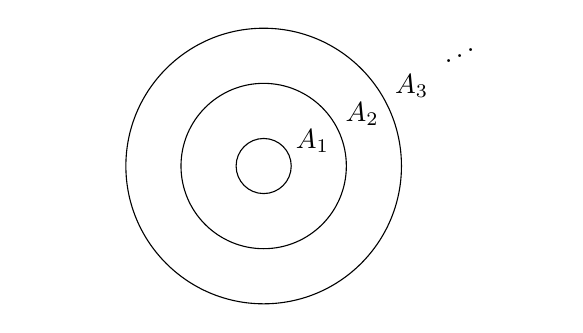
\begin{tikzpicture}[scale=0.7]
\draw (0,0) circle (0.5cm);
\draw (0,0) circle (1.5cm);
\draw (0,0) circle (2.5cm);
\node[text width=1cm] at (1.3,0.45) {$A_1$};
\node[text width=1cm] at (2.2,0.95) {$A_2$};
\node[text width=1cm] at (3.1,1.45) {$A_3$};
\node[text width=1cm] at (4.0,1.9) {.};
\node[text width=1cm] at (4.2,2.0) {.};
\node[text width=1cm] at (4.4,2.1) {.};
\node[text width=1cm] at (-3.4,2.1) {};
\end{tikzpicture}
\end{center}
\par
To illustrate, you can visualize $\{A_i\}_{i=1}^{\infty}$ in a Venn diagram as a sequence of disks, with each disk surrounding and \emph{including} those that came before. On the other hand, $\{E_i\}_{i=1}^{\infty}$ is the sequence of \emph{rings}, which don't overlap, so this sequence is mutually exclusive. Every outcome in $A_n$ is also in $E_n$, or in some $E_i$ with $i < n$, so $\cup_{i=1}^{n} A_i = \cup_{i=1}^{n} E_i$ for all $n$ (and $\cup_{i=1}^{\infty} A_i = \cup_{i=1}^{\infty} E_i$ for the same reason).
\eqns{P\left(\bigcup_{i=1}^{\infty}A_i\right) &= P\left(\bigcup_{i=1}^{\infty}E_i\right) = \sum_{i=1}^{\infty} P(E_i) = \lim_{n \to \infty} \sum_{i=1}^{n} P(E_i) = \lim_{n \to \infty} P\left(\bigcup_{i=1}^{n} E_i \right)}
\par
Note that the second equality is justified by axiom (iii), the third is the definition of an infinite sum, and the fourth is axiom (iii) being used again, this time in the opposite direction. To finish the argument, recall that $\cup_{i=1}^{n} A_i = \cup_{i=1}^{n} E_i$ and $\{A_i\}_{i=1}^{\infty}$ is an increasing sequence, so $\cup_{i=1}^{n} A_i = A_n$.
\eqns{\lim_{n \to \infty} P\left(\bigcup_{i=1}^{n} E_i \right) = \lim_{n \to \infty} P\left(\bigcup_{i=1}^{n} A_i \right) = \lim_{n \to \infty} P(A_n)}
\end{pf}

\begin{examp}
Suppose we pick a real number in the $[0,1]$ by choosing each of its decimal digits at random. What is the probability the number selected is $\frac{2}{9}$\,?
\par
If we let $T_i$ be the event  `the first $i$ digits are all twos', then the sequence $\{T_i\}_{i=1}^{\infty}$ is a decreasing sequence, and the event $\cap_{i=1}^{\infty}T_i$ occurs when all the $T_i$'s occur, i.e. when the number selected is $0.2222222... = \frac{2}{9}$\,. 
\eqns{P(T_1) = \frac{1}{10}, \ \ \ P(T_2) = \frac{1}{100} = \frac{1}{10^2}, \ \ \ P(T_3) = \frac{1}{1000} = \frac{1}{10^3}, \ \ \  ...}
\par
In general, $P(T_n) = \frac{1}{10^n}$, so by Theorem \ref{continuity} above (for decreasing sequences), the probability that the chosen number is $\frac{2}{9}$ is
\eqnsgap{P(\bigcap_{i=1}^{\infty} T_i) = \lim_{n \to \infty}P(T_n) = \lim_{n \to \infty} \frac{1}{10^n} = 0.}
\end{examp}
\par
This example illustrates the difference between an event with probability zero and an event which can never occur. If we choose a number in the interval $[0,1]$ at random, \emph{every possible outcome can be shown to have probability zero}.
\par
%This may sound strange, but there are infinitely many distinct outcomes, all of which must have the same probability of occurring. If that probability was any fixed positive number, the sum of these probabilities would be infinite, violating axioms (i) and (iii).
%\par
To get some intuition for why this is the case, suppose I've chosen a number, and you decide to confirm whether or not it's equal to $\frac{2}{9}$. You ask `does the first digit match', and I reply `yes'; you ask `does the second digit match', and I reply `yes'; and so on. If I have truly chosen each digit at random, then every time you ask about the next digit, I have a $\frac{9}{10}$ chance of replying `no', which will end the game immediately, and whenever I reply `yes' you simply challenge me again.
\par
Note that if we let $N_{\frac{2}{9}}$ denote the event `the number selected is not $\frac{2}{9}$', then by Corollary \ref{complementrule}, $P(N_{\frac{2}{9}}) = 1$. In fact, for any $x \in [0,1]$ if we define $N_x$ in the same way, then $P(N_x) = 1$ for all $x \in [0,1]$. Each event $N_x$ has probability 1, but it is certain that one of them will \emph{not} occur. We say that events with probability one \emx{almost surely}\index{Events!almost surely occurring} occur and events with probability zero \emx{almost never}\index{Events!almost never occurring} occur.
\par
\rmk The subtle distinction between an event with probability zero and an event which never occurs disappears in a finite sample space. In that case, an event with probability zero never occurs, and an event with probability one always occurs. 
\par
In any \emph{finite} number of trials of an experiment, you should expect an almost sure event to always occur, and an event which almost never occurs to actually never occur. This is the frequentist interpretation of events with probability one and probability zero. You should be willing to take a bet that an almost sure event will occur with \emph{any odds}, no matter how large the required wager and how small the potential gain. Conversely, you should never be willing to take a bet on an event which almost never occurs, no matter how small the required wager and how large the potential gain.

\section{Conditional Probability}\label{condprobsection}

Until now, our probability calculations have been done with no information other than a precise description of all possible outcomes of an experiment, given in the form of a sample space, and the assumption that certain events are equally likely, such as each of the six outcomes that can occur when a die is rolled.
\par
In practice, we are often given incomplete information about the result of an experiment, and we need to be able to update the probability that an event occurs when presented with this information. Consider the following examples.
\par
\begin{examp}Suppose a single die is rolled. We are not told the result, but we are told it was an even number. What is the probability the result was six? 
\par
Let $\Omega = \{1,2,3,4,5,6\}$, let $S =$ `the outcome was a six', and let $E =$ `the outcome was an even number'. Initially, each outcome in $\Omega$ is equally likely, and $P(S) = \frac{1}{6}$. However, given the knowledge that an even number was rolled, the sample space has been reduced from all the outcomes in $\Omega$ to only those in $E$. Now each of the three even outcomes are equally likely, and each of the odd outcomes has probability zero. We write $P(S \given E) = \frac{1}{3}$ to indicate the probability of $S$ under the assumption that $E$ has occurred is $\frac{1}{3}$.
\end{examp}
\begin{examp} In a certain school, 35\% of students receive an A grade in reading, 22\% of students receive an A grade in mathematics, and 16\% of students receive an A grade in both. Of those students who received an A grade in reading, what proportion also received an A grade in mathematics?
\par
\noindent Let the number of students at the school be denoted by $n$. Then the number that received an A in reading is $0.35n$, the number that received an A in mathematics is $0.22n$, and the number that received an A in both is $0.16n$. If we are considering only students who received an A in reading, we are dealing with a pool of $0.35n$ students. The only students in this pool who received an A in math must have received an A in both subjects, so there are total of $0.16n$ such students.
\par
\noindent Thus, the proportion of A students in reading who also received an A in math is $\frac{0.16n}{0.35n} = \frac{0.16}{0.35} \simeq 0.46 = 46\%$. Note that if we select a student at random and define the events $R =$ `the student received an A in reading' and $M =$ `the student received an A in math', then we can rewrite this calculation as
$$P(M \given R) = \frac{P(M \cap R)}{P(R)} = \frac{0.16}{0.35} \simeq 0.46.$$
\end{examp}
\par
We'll use this idea to formally define conditional probability, but it's often more productive to view conditional probability as a reduction of the sample space. In the example above, if you gathered \emx{only students who received an A in reading} in a room together and asked those who received an A in math to raise their hands, $46\%$ of them would raise their hands (if they're honest).
\par
\begin{defn}\label{conditionalprob}
Given two events $E$ and $F$ in some sample space $\Omega$, the conditional probability of $E$ given $F$\index{Conditional Probability} is denoted $P(E \given F)$, and defined by
\eqns{\boxed{P(E \given F) = \frac{P(E \cap F)}{P(F)}.}}
\end{defn}
Note that division by zero could be problematic here, so we'll only define the conditional probability of $E$ given $F$ when $P(F) \neq 0$.

\subsection*{The Intersection Law}\index{Intersection Law}

This definition can be used either to compute $P(E \given F)$ when $P(E \cap F)$ and $P(F)$ are known, or to compute $P(E \cap F)$ when $P(E \given F)$ and $P(F)$ are known. In fact, we'll often use it in this second way, so it's worth renaming some variables and moving terms around to make it easier to use in that direction.
\eqns{P(B \given A) &= \frac{P(B \cap A)}{P(A)} \\
P(B \given A) P(A) &= P(B \cap A) \\
P(B \given A) P(A) &= P(A \cap B)}
$$\boxed{P(A \cap B) = P(A) P(B \given A)}$$
\par
Intuitively, if $A$ and $B$ both occur, then $A$ must occur and $B$ must occur in this new setting where the event $A$ has already happened.
\begin{examp}
Suppose we draw two cards from a shuffled deck without replacement. What is the probability that both are hearts? 
\par
\noindent Let $H_1 =$ `the first card drawn is a heart' and $H_2 =$ `the second card drawn is a heart'. Then both cards are hearts when $H_1 \cap H_2$ occurs.
\eqnspar{P(H_1 \cap H_2) = P(H_1)P(H_2 \given H_1) = \frac{13}{52}\cdot\frac{12}{51} = \frac{156}{2652} \simeq 0.059}
\par
\noindent The key point is that if $H_1$ has occurred, a heart has been removed from the deck. There are then 51 cards remaining, 12 of which are hearts, so $P(H_2 \given H_1) = \frac{12}{51}$.
\end{examp}
\begin{examp}
Consider a point selected at random in a unit square, as in Example \ref{unitsquare}. We take $\Omega = \{(x,y) \, | \, 0 \leq x \leq 1 \text{ and } 0 \leq y \leq 1\}$. If the point has $x < y$, what is the probability it lies in the top third of the square?
\par
\noindent We're looking for $P(T \given G)$ where $T = \{(x,y) \, | \, 0 \leq x \leq 1 \text{ and } \frac{2}{3} \leq y \leq 1\}$ and $G = \{(x,y) \, | \, 0 \leq x < y \leq 1\}$. To compute this probability, we can draw a picture.

\begin{center}
\begin{minipage}{1.6in}
\begin{center}
\begin{tikzpicture}[scale=0.7]
\node (v1) at (-1.5,-1.5) {};
\node (v2) at (1.5,1.5) {};
\node (v3) at (-1.5,1.5) {};
\node (t) at (0,-0.5) {$G$};
\node (g) at (2,1) {$T$};
\draw (v1.center)--(v2.center)--(v3.center);
\fill [pattern=north west lines, pattern color=black] (v1.center)--(v2.center)--(v3.center);
\draw (-1.5,-1.5) rectangle (1.5,1.5);
\draw (-1.5,0.5) rectangle (1.5,1.5);
\fill [pattern=north east lines, pattern color=black] (-1.5,0.5) rectangle (1.5,1.5);
\end{tikzpicture}
\end{center}
\end{minipage}
\end{center}
\vspace{0pt}

\noindent The square has unit area, and hence the area of any region inside it represents the probability a randomly selected point will lie in that region. 
\eqns{P(T \cap G) = \frac{1}{3} - \frac{1}{18} = \frac{5}{18} \text{\ \  and \ } P(G) = \frac{1}{2}}
\par
\noindent Therefore, $P(T \given G) = \displaystyle\frac{P(T \cap G)}{P(G)} = \frac{\frac{5}{18}}{\frac{1}{2}} = \frac{5}{9}$.
\end{examp}

As an application of these ideas, let's analyze a classic puzzle presented by Martin Gardner \cite{TwoChild}. Consider the two statements below.
\vspace*{-4pt}
\begin{enumerate}
\item Mr.\,Jones has two children. The older child is a girl. What is the probability his other child is a girl?
\item Mr.\,Smith has two children. At least one is a girl. What is the probability the other child is a girl?
\end{enumerate}
\par
Answering the first question is relatively straightforward. Consider the sample space $\Omega = \{bb, bg, gb, gg\}$, the first letter representing the gender of the elder child, and the second letter representing the gender of the younger. Given no information about Mr.\,Jones' family, each outcome in this sample space is equally likely. If we let $E =$ `the elder child is a girl' and $Y =$ `the younger child is a girl', then
\eqnspar{P(Y \given E) = \frac{P(Y \cap E)}{P(E)} = \frac{\frac{1}{4}}{\frac{1}{2}} = \frac{1}{2}.}
\par
Which agrees with intuition. The second question involving Mr.\,Smith's family is more problematic. On the one hand, we could let $A =$ `at least one child is a girl' and $B =$ `both children are girls', and calculate
\eqnspar{P(B \given A) = \frac{P(B \cap A)}{P(A)} = \frac{\frac{1}{4}}{\frac{3}{4}} = \frac{1}{3}.}
\par
On the other hand, without any information, a given child is equally likely to be a boy or girl, and the fact that one child is a girl gives us no information about Mr. Smith's  \emph{other child}, so the chance that second child is a girl should still be $\frac{1}{2}$.
\par
Which is correct, $\frac{1}{3}$ or $\frac{1}{2}$? The key to resolving the paradox is to clarify what experiment is actually being performed. If we \emx{choose at random a family} with two children, one of which is a girl, the three possibilities $bg$, $gb$, and $gg$ are equally likely, and our calculation of $P(B \given A)$ above is correct. 
\par
However, if we \emx{choose at random a girl} from a family with two children, a $bg$ or $gb$ family is half as likely to be chosen as a $gg$ family, since the latter has twice as many girls! Thus, $P(\{bg\}) = P(\{gb\}) = \frac{1}{4}$, and $P(\{gg\}) = \frac{1}{2}$. In this context, the event $A =$ `at least one child is a girl' always occurs, and we can calculate
\eqnspar{P(B \given A) = \frac{P(B \cap A)}{P(A)}  = \frac{\frac{1}{2}}{1}= \frac{1}{2}.}
\par
The moral of the story is that we need to specify the experiment being performed and the source of uncertainty; in this case, the process by which Mr.\,Smith's family was chosen. When you read `Mr.\,Smith has two children', you should immediately ask who Mr.\,Smith is and how he was chosen. Without this information, the second question is ambiguous.

\subsection*{Extending the Intersection Law}

We've derived the intersection law $P(A \cap B) = P(A) P(B \given A)$ from the definition of conditional probability. It's worth noting that this law generalizes to intersections of any number of events,
\eqnspar{P(A_1 \cap A_2 \cap A_3 \cap ...) = P(A_1) P(A_2 \given A_1) P(A_3 \given A_1 \cap A_2)\, ... }
\par
\noindent where each factor on the right is the conditional probability of $A_i$ calculated under the assumption that all prior events in the sequence have occurred.
\begin{examp}
What is the probability that when we draw four cards from a deck without replacement, all four cards are different suits?
\par
\noindent Let $D_i =$ `the $i^{th}$ card is a different suit from all those cards the came before', then $P(D_1) = 1$, since no cards were drawn before the first, and we calculate
\eqns{P(D_1 \cap D_2 \cap D_3 \cap D_4) &= P(D_1)P(D_2 \given D_1)P(D_3 \given D_1 \cap D_2)P(D_4 \given D_1 \cap D_2 \cap D_3) \\
&= 1 \cdot \frac{39}{51} \cdot \frac{26}{50} \cdot \frac{13}{49} \simeq 0.1055}

\end{examp}
\begin{examp}
Suppose that seven lightbulbs are in a box, but only two work. Bob will randomly select lightbulbs one at a time and test them. What is the probability he'll find both working lightbulbs after exactly three tests?
\par
\noindent Let $W_i =$ `the $i^{th}$ lightbulb tested works'. Then we need $W_3$ to occur, and one of $W_1$ and $W_2$. If $W_1$ and $W_2$ both occur then Bob will be finished after only two tests.
\eqns{&P((W_1 \cap {W_2}^c \cap W_3) \cup ({W_1}^c \cap W_2 \cap W_3)) \\
&= P(W_1 \cap {W_2}^c \cap W_3) + P({W_1}^c \cap W_2 \cap W_3) \\
&= P(W_1)P({W_2}^c \given W_1)P(W_3 \given W_1 \cap {W_2}^c) + P({W_1}^c)P(W_2 \given {W_1}^c)P(W_3 \given {W_1}^c \cap W_2) \\
&= \frac{2}{7}\cdot\frac{5}{6}\cdot\frac{1}{5} + \frac{5}{7}\cdot\frac{2}{6}\cdot\frac{1}{5} = \frac{10}{210} + \frac{10}{210} \simeq 0.095}
\par
\noindent Note that $W_1 \cap {W_2}^c \cap W_3$ and ${W_1}^c \cap W_2 \cap W_3$ are mutually exclusive, so we can pass from the first to the second line without using the inclusion-exclusion principle.
\end{examp}

\subsection*{Conditional Probability is Well-Behaved}

Interpreting conditional probability as a reduction of the sample space from $\Omega$ to some $B \subseteq \Omega$ with $P(B) > 0$, it's not hard to convince yourself that the Kolmogorov axioms hold for events conditioned on the occurrence of $B$. The meaning of each axiom is the same, it's just being interpreted in the smaller sample space $B$.
\begin{enumerate}
\item $P(A \given B) \geq 0$.
\item $P(B \given B) = 1$.
\vspace*{-7pt}
\item If $\{A_i\}_{i=1}^{\infty}$ is mutually exclusive, $P\displaystyle\left(\left. \bigcup_{i=1}^{\infty} A_i \,\right|\, B \right) = \sum_{i=1}^{\infty} P(A_i \given B)$.
\end{enumerate}
\par
This implies that \emx{all the laws we derived in Section \ref{probaxiomssection} apply for conditional probabilities as well}. The inclusion-exclusion law, for example, can be written for events $A$ and $B$ conditioned on $C$ as
\eqnsgap{P(A \cup B \given C) = P(A \given C) + P(B \given C) - P(A \cap B \given C).}
\begin{examp}
Suppose that in a certain area, 36\% of all cats are black, and 76\% of all black cats are mean. What is the probability that a randomly selected cat is black and not mean?
$$P(B \cap M^c) = P(B)P(M^c \given B) = P(B)(1-P(M \given B)) = 0.36 \cdot 0.24 = 0.0864$$
\end{examp}
\par
\rmk If you read up on conditional probability, you might encounter notation such as $P(A \given B,C)$. This means we are assuming all events on the right side of the vertical line have occurred, so $P(A \given B,C) = P(A \given B \cap C)$.

\section{The Law of Total Probability}

If two cards are drawn from a shuffled deck, what is the probability the second card drawn is a heart? At first, it's tempting to reply that in order to answer, we would require more information, namely, whether the first card drawn was a heart or not.
\par
However, recalling the frequentist interpretation, the question above is perfectly well posed. If we repeat the experiment a very large number of times, then in some proportion of trials, the second card will be heart. In order to compute this value analytically, we'll need the result below.
\par
\begin{thm}\label{lawtotalprob}\index{Law of Total Probability}
(Law of Total Probability) If $\{A_i\}_{i=1}^{n}$ is any mutually exclusive sequence of events with $\bigcup_{i=1}^{n}A_i = \Omega$, then for any event $B$,
$$\boxed{P(B) = P(B \given A_1)P(A_1) + P(B \given A_2)P(A_2)+ \, ... \, + P(B \given A_n)P(A_n).}$$
\noindent Note that we require $P(A_i) > 0$ for each $A_i$, so that the conditional probabilities on the right are defined.
\end{thm}
\par
When a sequence $\{A_i\}_{i=1}^{n}$ is mutually exclusive and has $\bigcup_{i=1}^{n}A_i = \Omega$, we say that the sequence \emx{partitions the sample space}. This means that every possible outcome is in exactly one of the $A_i$.

\begin{center}
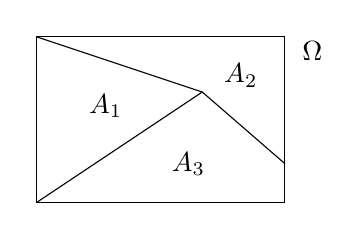
\begin{tikzpicture}[scale=0.7]
\draw (-1.5,-1.5) rectangle (3.0,1.5);
\node (O) at (3.5,1.25) {$\Omega$};
\node (v1) at (-1.5,-1.5) {};
\node (v2) at (1.5,0.5) {};
\node (v3) at (-1.5,1.5) {};
\node (v4) at (3.0,-0.8) {};
\node (a1) at (-0.25,0.25) {$A_1$};
\node (a2) at (2.2,0.8) {$A_2$};
\node (a3) at (1.25,-0.8) {$A_3$};
\draw (v1.center)--(v2.center)--(v3.center);
\draw (v4.center)--(v2.center);
\end{tikzpicture}
\end{center}

\begin{cor} If $A$ is an event with $0 < P(A) < 1$, then for any event $B$, 
\eqnsgap{\boxed{P(B) = P(B \given A)P(A) + P(B \given A^c)P(A^c).}}
\end{cor}
\begin{pf} Apply Theorem \ref{lawtotalprob} to the sequence $\{A, A^c\}$, which always partitions $\Omega$.
\end{pf}

\begin{examp}
If two cards are drawn from a shuffled deck, what is the probability the second card drawn is a heart?
\par
\noindent Let $H_1 =$ `the first card is a heart' and $H_2 =$ `the second card is a heart'. We'll apply the corollary above to compute the probability of $H_2$.
\eqns{P(H_2) &= P(H_2 \given H_1)P(H_1) + P(H_2 \given {H_1}^c)P({H_1}^c) \\ &= \frac{12}{51} \cdot \frac{1}{4} + \frac{13}{51} \cdot \frac{3}{4} = \frac{51}{204} = \frac{1}{4}}
\par
\noindent This result makes intuitive sense. We're computing $P(H_2)$ in the absence of any information about the first card, so we may as well have drawn that card and put it on the bottom of the deck without looking at it.
\end{examp}
\begin{pf} (of Theorem \ref{lawtotalprob}) If the sequence $\{A_i\}_{i=1}^n$ partitions $\Omega$, and $B \subseteq \Omega$,
\eqns{\Omega &= A _1 \cup A_2 \cup \, ... \, \cup A_n \\ B \cap \Omega &= B \cap (A_1 \cup A_2 \cup \, ... \, \cup A_n) \\ B &= (B \cap A_1) \cup (B \cap A_2) \cup \, ... \, \cup (B \cap A_n).}
\par
\noindent The sequence of events $B \cap A_1, B \cap A_2, \, ... \,, B \cap A_n$ is mutually exclusive because $\{A_i\}_{i=1}^{n}$ was mutually exclusive, and this new sequence is obtained by reducing the number of outcomes in each event. The events had empty intersections initially, so removing outcomes will keep the intersections empty.
\eqns{P(B) &= P((B \cap A_1) \cup (B \cap A_2) \cup \, ... \, \cup (B \cap A_n)) \\ &= P(B \cap A_1) + P(B \cap A_2) + \, ... \, + P(B \cap A_n) \\ &= P(A_1 \cap B) + P(A_2 \cap B) + \, ... \, + P(A_n \cap B) \\ &= P(A_1)P(B \given A_1) + P(A_2) P(B \given A_2) + \, ... \, + P(A_n) P(B \given A_n)\\ &= P(B \given A_1)P(A_1) + P(B \given A_2)P(A_2)  + \, ... \, + P(B \given A_n)P(A_n)}
\end{pf}

\subsection*{Tree Diagrams}\index{Tree Diagram}

Tree diagrams are a nice graphical tool for organizing calculations, and have the law of total probability built in to their structure. Each column represents a step in an experiment. If we draw three balls from an urn, for example, each column will represent a draw. If we roll a die and then flip a coin, the first column will represent the roll and the second will represent the flip.

\begin{examp}
What is the probability that, when three cards are drawn from a shuffled deck without replacement, exactly one heart appears?
\par
\noindent In the tree diagram below, the three columns represent three draws from a deck of cards, when a draw results in a heart, we denote that with an $H$, and when a draw does not result in a heart, we denote that with an $N$.
\begin{center}
\begin{tikzpicture}[grow=right]
\node[bag] {.}
    child {
        node[bag] {N}        
            child {
                node[bag]{N}
                    child {
                     node[bag] {$H \qquad \frac{1482}{10200}$}
                     edge from parent
                     node[above]  {$\frac{13}{50}$}
                    }
                edge from parent
                node[below]  {$\frac{38}{51}$}
            }
            child {
                node[bag]{H}
                    child {
                     node[bag] {$N \qquad \frac{1482}{10200}$}
                     edge from parent
                     node[above]  {$\frac{38}{50}$}
                 }
                edge from parent
                node[above]  {$\frac{13}{51}$}
            }
            edge from parent 
            node[below]  {$\frac{3}{4}$}
    }
    child {
        node[bag] {H}        
        child {
            node[bag] {N}
                child {
                     node[bag] {$N \qquad \frac{1482}{10200}$}
                     edge from parent
                     node[above]  {$\frac{38}{50}$}
                 }
                edge from parent
                node[above]  {$\frac{39}{51}$}
         }
        edge from parent         
            node[above]  {$\frac{1}{4}$}
    };
\end{tikzpicture}
\end{center}
\par
\noindent Each edge is labelled with a conditional probability. For example, the top-center edge which runs from $H$ to $N$ is labelled with $P(N_2 \given H_1)$, the probability a non-heart is drawn on the second draw, after drawing a heart on the first. Note that we only depict the branches where the desired event (`at least one heart appears') occurs. To find the probability of this event, we simply multiply along each branch, and add the results. If $E =$ `exactly one heart is drawn', then
\eqnsgap{P(E) = \frac{1482}{10200} + \frac{1482}{10200} + \frac{1482}{10200} = \frac{4446}{10200} \simeq 43.6\%.}
\end{examp}
\par
This approach works because the branches represent mutually exclusive events (at each fork, a given trial of the experiment can proceed along only one path), so we can add the probabilities of each branch. Furthermore, the intersection law states that we can compute the probability of all events along a branch occurring by multiplying their conditional probabilities as we did above. Note that if we applied the law of total probability in the above example, partitioning the sample space with $\{H_1 \cap H_2, H_1 \cap N_2, N_1 \cap H_2, N_1 \cap N_2\}$, we would obtain
\eqns{P(E) =& \ P(E \given H_1 \cap H_2)P(H_1 \cap H_2) + P(E \given H_1 \cap N_2)P(H_1 \cap N_2) \\ &+ P(E \given N_1 \cap H_2)P(N_1 \cap H_2) + P(E \given N_1 \cap N_2)P(N_1 \cap N_2) \\
=& \ 0 + P(E \given H_1 \cap N_2)P(N_2 \given H_1)P(H_1) + P(E \given N_1 \cap H_2)P(H_2 \given N_1)P(N_1) \\ &+ P(E \given N_1 \cap N_2)P(N_2 \given N_1)P(N_1) \\
=& \ P(N_3 \given H_1 \cap N_2)P(N_2 \given H_1)P(H_1) + P(N_3 \given N_1 \cap H_2)P(H_2 \given N_1)P(N_1) \\ &+ P(H_3 \given N_1 \cap N_2)P(N_2 \given N_1)P(N_1)}
\par
\noindent and this is exactly how we calculated the result above. Each path from left to right corresponds to a term in the sum above. The event $E$ never occurs if two hearts are drawn, so $P(E \given H_1 \cap H_2) = 0$ and that term (which corresponds to a branch not depicted in the diagram) vanishes. Although working through the notation is good practice, I expect you'll agree that in cases like this, the tree diagram is more intuitive and simplifies the bookkeeping.
\par
If at any point in the tree diagram, the event we're interested in is sure to occur, there's no need to continue along that branch any further. We can save time in this way, as illustrated in the example below.
\begin{examp}
Suppose that an urn contains three red and five green balls. If three balls are drawn from the urn without replacement, what is the probability that at least one red ball will be drawn?
\tikzstyle{level 1}=[level distance=2.5cm, sibling distance=1.5cm]
\begin{center}
\begin{tikzpicture}[grow=right]
\node[bag] {.}
    child {
        node[bag] {G}        
            child {
                node[bag]{G}
                    child {
                     node[bag]{$R \qquad \frac{60}{336}$}
                     edge from parent
                     node[below]  {$\frac{3}{6}$}
                    }
                edge from parent
                node[below]  {$\frac{4}{7}$}
            }
            child {
                node[bag]{$R \qquad \frac{15}{56}$}
                edge from parent
                node[above]  {$\frac{3}{7}$}
            }
            edge from parent 
            node[below]  {$\frac{5}{8}$}
    }
    child {
        node[bag]{$R \qquad \frac{3}{8}$}        
        edge from parent         
            node[above]  {$\frac{3}{8}$}
    };
\end{tikzpicture}
\tikzstyle{level 1}=[level distance=2.5cm, sibling distance=2.25cm]
\end{center}
\par
\noindent As soon as a red ball is drawn, there's no need to continue the branch. Regardless of what happens from that point on, a red ball will have been drawn. If A = `at least one red ball is drawn', then 
\eqnsgap{P(A) = \frac{3}{8} + \frac{15}{56} + \frac{60}{336} = \frac{276}{336} \simeq 82.1\%.}
\end{examp}
\begin{examp}
Suppose we draw cards with replacement from a shuffled deck until the first ace appears. What is the probability that all cards drawn are black?
\tikzstyle{level 1}=[level distance=2.5cm, sibling distance=1.5cm]
\begin{center}
\begin{tikzpicture}[grow=right]
\node[bag] {.}
    child {
        node[bag] {BNA}        
            child {
                node[bag]{BNA}
                    child {
                     node[bag]{$...$}
                     edge from parent
                     node[below]  {$\frac{24}{52}$}
                    }
										child {
                     node[bag]{$BA$}
                     edge from parent
                     node[above]  {$\frac{2}{52}$}
                    }
                edge from parent
                node[below]  {$\frac{24}{52}$}
            }
            child {
                node[bag]{$BA$}
                edge from parent
                node[above]  {$\frac{2}{52}$}
            }
            edge from parent 
            node[below]  {$\frac{24}{52}$}
    }
    child {
        node[bag]{$BA$}        
        edge from parent         
            node[above]  {$\frac{2}{52}$}
    };
\end{tikzpicture}
\tikzstyle{level 1}=[level distance=2.5cm, sibling distance=2.25cm]
\end{center}
\par
\noindent Here $BA$ denotes `black ace' and $BNA$ denotes `black non-ace'. There's no limit to the number of draws that could occur before the first black ace appears, so the tree diagram is infinite. However, we can still sum the products along each branch. Let $OB = $ `only black cards are drawn', then
\eqnsgap{P(OB) &= \frac{2}{52} + \frac{24}{52}\cdot\frac{2}{52} + \frac{24}{52}\cdot\frac{24}{52}\cdot\frac{2}{52} +  \frac{24}{52}\cdot\frac{24}{52}\cdot\frac{24}{52}\cdot\frac{2}{52} + \ ... \\ 
&= \frac{2}{52}\left(1 + \frac{24}{52} + \left(\frac{24}{52}\right)^2 + \left(\frac{24}{52}\right)^3 + \ ...\right) \\
&= \frac{2}{52}\left(\sum_{i=0}^{\infty} \left(\frac{24}{52}\right)^n\right) \\
&= \frac{2}{52} \cdot \frac{1}{1-(\frac{24}{52})} = \frac{1}{14} \simeq 7.1\%}
\end{examp}
\par
Note that the sum of the infinite series above was evaluated with the geometric series sum formula, $a+ar+ar^2+ ... = \frac{a}{1-r}$ when $-1 < r < 1$.

\section{Independence}\index{Independence}\label{IndependenceOfEvents}

Suppose we flip a coin and then roll a die. Let $H$ denote the event `a head is flipped', $E$ denote the event `and even number is rolled' and $L$ denote the event `a number larger than three was rolled'. Note that
$$P(E) = \frac{1}{2} \text{ \ and \ } P(E \given H) = \frac{1}{2}.$$
Knowledge that a head was flipped doesn't change the probability an even number was rolled. On the other hand, we can calculate 
$$P(E) = \frac{1}{2} \text{ \ and \ } P(E \given L) = \frac{2}{3}.$$
In this case, knowledge that the number rolled was a four, five, or six increases the probability that the result of the roll was even. The events $E$ and $H$ are said to be \emx{independent}, while the events $E$ and $L$ are \emx{not independent}.
\begin{defn}\label{independentevents}
Events $A$ and $B$ are called independent\index{Events!independent}\index{Independence!of a pair of events} if $P(B) = P(B \given A)$.
\end{defn}
\begin{examp}Suppose we flip a coin two times. Note that $\Omega = \{HH, HT, TH, TT\}$ is a sample space with equally likely outcomes for the experiment.
\par
\noindent If we consider the events $H_1 =$ `the first flip is a head' and $H_2 =$ `the second flip is a head', then $P(H_2) = \frac{1}{2}$ and $P(H_2 \given H_1) = \frac{1}{2}$, so these events are independent.
\par
\noindent If we instead let $H_1 =$ `the first flip is a head' and $T_1 =$ `the first flip is a tail', then $P(T_1) = \frac{2}{4}$ and $P(T_1 \given H_1) = 0$, so these two events are not independent.
\end{examp}
\begin{examp}
Consider two cards drawn from a shuffled deck. Let $S_1 =$ `a spade is drawn on the first draw' and $S_2 =$ `a spade is drawn on the second draw'. Then $S_1$ and $S_2$ are independent provided the draws are done with replacement, but not independent if the draws are done without replacement. In this second case, $P(S_2 \given S_1) = \frac{12}{51}$, but using the law of total probability, $P(S_2) = \frac{1}{4}$.
\end{examp}
\par
Using the definition of the conditional probability $P(A \given B)$, we can state what it means for two events to be independent in a different way. 
$$P(A) = P(A \given B) \biimp P(A) = \frac{P(A \cap B)}{P(B)} \biimp P(A)P(B) = P(A \cap B)$$
Thus, when $A$ and $B$ are independent events, $P(A \cap B) = P(A)P(B)$. This relation is often used as the definition of independence. As we just saw, it's equivalent to the definition we gave earlier but also applies when $P(A) = 0$ or $P(B) = 0$ (in these cases $P(A\given B)$ or $P(B \given A)$ would be undefined).

\rmk Independence is a symmetric relation, which you can interpret intuitively as saying `the probability of one event occurring is not influenced by the occurrence of the other' without worrying about which event comes first. This revised definition shows that intuition is correct, as exchanging the letters $A$ and $B$ gives yields the same equation.
\begin{thm}\label{compindependent}
If $A$ and $B$ are independent, then $A$ and $B^c$ are independent.
\end{thm}
\begin{pf}
Note that $A = (A \cap B) \cup (A \cap B^c)$ and hence $P(A) = P(A \cap B) + P(A \cap B^c)$ since the two events on the right are mutually exclusive. Isolating $P(A \cap B^c)$,
\eqns{P(A \cap B^c) &= P(A) - P(A \cap B) \\
&= P(A) - P(A)P(B) \\
&=P(A)(1-P(B)) \\
&= P(A)P(B^c).}
\end{pf}
\begin{cor}
If $A$ and $B$ are independent, then $A^c$ and $B^c$ are independent.
\end{cor}
\begin{pf}
If $A$ and $B$ are independent, then $A$ and $B^c$ are independent by Theorem \ref{compindependent}, but independence is symmetric, so applying Theorem \ref{compindependent} again, this time to $B^c$ and $A$, we conclude $B^c$ and $A^c$ are independent.
\end{pf}
\par
Given a sequence of events $\{A_1, A_2, \, ... \, , A_n\}$, we say this sequence is independent if the occurrence of any collection of these events does not influence the chance that any other event in the sequence occurs. Formally, it's easiest to state this by extending the relation $P(A \cap B) = P(A)P(B)$ to arbitrary subsets of the sequence.
\begin{defn}\index{Independence!of a sequence of events}
The sequence of events $\{A_i\}_{i=1}^{n}$ is independent if for any collection $\{A_{i_1}, A_{i_2}, \, ... \, , A_{i_k}\}$ of events taken from the sequence,
\eqnsgap{P(A_{i_1} \cap A_{i_2} \cap \, ... \, \cap A_{i_k}) = P(A_{i_1})P(A_{i_2}) \, ... \, P(A_{i_k})}
\end{defn}
\begin{examp}
Suppose we toss a fair coin twice. Let $H_1 =$ `The first toss is heads', $H_2 =$ `The second toss is heads', and $E =$ `Exactly one toss results in heads'. As we already observed, $H_1$ and $H_2$ are independent. Moreover, $P(E) = \frac{1}{2}$ since exactly one head is flipped in two of the four equally likely outcomes, and $P(E \given H_1) = \frac{1}{2}$ since assuming $H_1$ occurs, $E$ occurs when the second flip is a tail. Thus, $H_1$ and $E$ are independent, and essentially the same argument shows $H_2$ and $E$ are independent.
\par
\noindent Since each pair of events in the sequence $\{H_1, H_2, E\}$ is independent, we say this sequence is pairwise independent\index{Pairwise Independence}. However, note that if we assume both $H_1$ and $H_2$ occur, the probability $E$ occurs becomes zero, that is, $P(H_1 \cap H_2 \cap E) = 0$, but we can calculate $P(H_1)P(H_2)P(E) = \frac{1}{2}\cdot\frac{1}{2}\cdot\frac{1}{2} = \frac{1}{8}$.
\end{examp}
\par
The example above illustrates that even if every pair of events in a sequence is independent, there could still be some event in the sequence whose probability is influenced by the joint occurrence of some larger collection of other events. In other words, for sequences of events, pairwise independence does not imply independence.
\par
\begin{examp}
Suppose that a 64 bit sequence (a sequence of 64 zeros and ones) is sent over an unreliable channel. The probability that each bit gets flipped is 0.005 independent of what happens to the other bits. What is the probability that the entire sequence is received without errors?
\par
\noindent Let $F_i = $ `the $i^{th}$ bit gets flipped', then $P(F_i) = 0.005$, and the probability that the $i^{th}$ bit is received correctly is $P({F_i}^c) = 1-0.005 = 0.995$. If $E =$ `the entire string is received without any flipped bits' then
\eqnsgap{P(E) &= P({F_1}^c \cap {F_2}^c \cap \, ... \, \cap {F_{64}}^c) \\
&= P({F_1}^c)P({F_2}^c) \, ... \, P({F_{64}}^c) \\
&= 0.995 \cdot 0.995 \cdot \, ... \, \cdot 0.995 \\
&\simeq 0.72556 \simeq 72.6\% } 
\end{examp}

\section{Bayes' Rule}

The tools of conditional probability have so far been used to find the probability of observing a particular outcome under some assumptions about the experiment being performed. In practice though, the problem is often the other way around. We observe a particular outcome, and we'd like to use that information as evidence to evaluate or update our assumptions about the internal workings of the experiment.
\begin{examp}\label{BayesUrn}
Two balls are drawn with replacement from an urn which contains either only red balls, or an equal number of red and green balls. The choice of how to load the urn is made by flipping a fair coin. If the experiment is performed, and both balls drawn are red, what is the probability the urn contains only red balls?
\noindent Consider the tree diagram given below, where every possible outcome is illustrated.
\begin{center}
\tikzstyle{level 1}=[level distance=3.5cm, sibling distance=2.5cm]
\tikzstyle{level 2}=[level distance=3.5cm, sibling distance=1.75cm]
\tikzstyle{level 3}=[level distance=2.5cm, sibling distance=0.75cm]
\begin{tikzpicture}[grow=right]
\node[bag] {.}
    child {
        node[bigbag] {All Red \\ Urn}        
            child {
                node[bag]{R}
                    child {
                     node[bag] {$R$}
                     edge from parent
                     node[below]  {$1$}
                    }
                edge from parent
                node[below]  {$1$}
            }
            edge from parent 
            node[below]  {$\frac{1}{2}$}
    }
    child {
        node[bigbag] {Red/Green Urn}        
        child {
            node[bag] {G}
                child {
                     node[bag] {$G$}
                     edge from parent
                     node[below]  {$\frac{1}{2}$}
                 }
                 child {
                     node[bag] {$R$}
                     edge from parent
                     node[above]  {$\frac{1}{2}$}
                 }
                edge from parent
                node[above]  {$\frac{1}{2}$}
         }
         child {
            node[bag] {R}
                child {
                     node[bag] {$G$}
                     edge from parent
                     node[below]  {$\frac{1}{2}$}
                 }
                 child {
                     node[bag] {$R$}
                     edge from parent
                     node[above]  {$\frac{1}{2}$}
                 }
                edge from parent
                node[above]  {$\frac{1}{2}$}
         }
        edge from parent         
            node[above]  {$\frac{1}{2}$}
    };
\end{tikzpicture}
\end{center}
\par
\noindent Now we know that two red balls were drawn, so let's reduce our sample space by disregarding all branches where this event doesn't occur. The updated tree diagram is given below.
\begin{center}
\tikzstyle{level 1}=[level distance=3.5cm, sibling distance=1.75cm]
\tikzstyle{level 2}=[level distance=3.5cm, sibling distance=1.75cm]
\tikzstyle{level 3}=[level distance=2.5cm, sibling distance=0.75cm]
\begin{tikzpicture}[grow=right]
\node[bag] {.}
    child {
        node[bigbag] {All Red \\ Urn}        
            child {
                node[bag]{R}
                    child {
                     node[bag] {$R \qquad \frac{1}{2}$}
                     edge from parent
                     node[below]  {$1$}
                    }
                edge from parent
                node[below]  {$1$}
            }
            edge from parent 
            node[below]  {$\frac{1}{2}$}
    }
    child {
        node[bigbag] {Red/Green Urn}        
         child {
            node[bag] {R}
                 child {
                     node[bag] {$R \qquad \frac{1}{8}$}
                     edge from parent
                     node[above]  {$\frac{1}{2}$}
                 }
                edge from parent
                node[above]  {$\frac{1}{2}$}
         }
        edge from parent         
            node[above]  {$\frac{1}{2}$}
    };
\end{tikzpicture}
\end{center}
Intuitively, since the top branch has a $\frac{1}{8}$ chance of occurring, and the bottom branch has a $\frac{1}{2}$ chance of occurring, the bottom branch is four times more likely to have occurred. Thus, there is a $\frac{4}{5}$ chance that the all red urn was being used, and a $\frac{1}{5}$ chance the urn with an equal number of red and green balls was being used.
\par
\noindent Formally, if we let $A =$ `the urn contains all red balls' then $A^c =$ `the urn contains and equal number of red and green balls', and we're looking for $P(A \given R_1 \cap R_2)$. Using the definition of conditional probability and the law of total probability,
\eqnsgap{P(A \given R_1 \cap R_2) &= \frac{P(A \cap R_1 \cap R_2)}{P(R_1 \cap R_2)} \\
&= \frac{P(A \cap R_1 \cap R_2)}{P(R_1 \cap R_1 \given A)P(A) + P(R_1 \cap R_2 \given A^c)P(A^c)} \\
&= \frac{\frac{1}{2} \cdot 1 \cdot 1}{1\cdot \frac{1}{2}+\frac{1}{4} \cdot \frac{1}{2}} = \frac{\frac{1}{2}}{\frac{1}{2} + \frac{1}{8}} = \frac{4}{5}.}
\end{examp}
\par
Initially, the chance the all red urn was selected was $\frac{1}{2}$. This belief was justified by the description of the experiment (whether or not the all red urn was selected was determined by a coin flip). After observing the results of a few draws, we were able to update our beliefs, and the chance the red urn was being used increased to $\frac{4}{5}$. The process of starting from some belief about the state of the world, and updating that beliefs based on new information is, essentially, learning.
\par
The facts we used to justify our conclusion were all derived from the Kolmogorov probability axioms, so the correctness of this approach, which is formalized in Bayes' rule below, is not in question. The fact that we can formalize the process of learning from new information is remarkable, and utility of this result is clear. From automated movie recommendations that change based on your ratings, to self-driving cars that get better at recognizing dangerous situations every time a crash happens, if you want to formalize the process of learning from new data, Bayes' rule is the fundamental tool.
\par
\begin{thm}\label{BayesRule}\index{Bayes' Rule}
(Bayes' Rule) For any events $A$ and $B$ in some sample space $\Omega$,
\eqnsgap{\boxed{P(A \given B) = \frac{P(B \given A)P(A)}{P(B)}}}
\end{thm}
\par
\begin{pf} We can derive Bayes' rule from the definition of conditional probability by applying the intersection rule in the numerator.
\eqns{P(A \given B) &= \frac{P(A\cap B)}{P(B)} = \frac{P(A)P(B \given A)}{P(B)}} 
\end{pf}
\par
It's worth noting that Bayes' rule, the intersection law, and the definition of conditional probability are essentially three different rearrangements of the same statement. These three different ways of thinking about one idea (the concept of conditional probability) lend themselves more naturally to different applications.
\par
Bayes' rule is shown in a compact form above. However in many applications, we will end up splitting the denominator into cases using the law of total probability.
\begin{cor}If $\{A_i\}_{i=1}^n$ is a sequence of events which partitions the sample space $\Omega$, and $B$ is an event,
\eqnsgap{\boxed{P(A_i \given B) = \frac{P(B \given A_i)P(A_i)}{P(B \given A_1)P(A_1) + \, ... \, + P(B \given A_n)P(A_n)}}}
\end{cor}
\begin{pf}
Apply Bayes' rule as presented in Theorem \ref{BayesRule} to the events $A_i$ and $B$, then expand the denominator using the law of total probability.
\end{pf}
\par
This expanded form of Bayes' rule closely matches the reasoning we did with tree diagrams in Example \ref{BayesUrn} above. In the numerator, we have the probability of the branch on which both the event we're assessing the probability of and the evidence we've observed occur, while in the denominator we have the sum of the probabilities of all the branches where the evidence we've observed occurs.
\begin{examp}
Suppose that a rare disease affects $0.5\%$ of the population. There is a test for this disease which is $99\%$ accurate, in the sense that the probability of a positive test for someone who carries the disease (a true positive) is $99\%$, and probability of a positive test for someone who does not carry the disease (a false positive) is 1\%. If an individual is randomly selected from the population and tests positive, what is the probability they have the disease?
\par
\noindent Let $D =$ `the randomly selected individual tested carries the disease', and $P =$ `the result of the test is positive'. Using Bayes' rule, we compute
\eqns{P(D \given P) &= \frac{P(P \given D)P(D)}{P(P \given D)P(D) + P(P \given D^c)P(D^c)} \\
&= \frac{0.99 \cdot 0.005}{0.99 \cdot 0.005 + 0.01 \cdot 0.995} \simeq 0.33.}
\par
\noindent Thus, if a randomly selected individual tests positive, there's a $33\%$ chance that they carry the disease. Despite the positive test result, the scenario where this individual does not carry the disease is still the more likely one. 
\end{examp}
\par
This example illustrates the problem of over-testing. If data from medical tests is to be useful, they should be applied carefully, often only in cases where there's some reason to believe the patient has an elevated risk of carrying the disease. As the test is more widely applied, the disease becomes more unusual in the group being tested and false positives become more likely. To illustrate this point, consider the most extreme case, where we're testing for a disease which has no cases in the group being tested. Every positive test will be a false positive, regardless of how well-designed the test might be. The utility of any test is a function of not just the intrinsic properties of the test, but also of the nature of the environment in which the test is being applied. 
\par
Assessing the usefulness of a procedure by examining only its intrinsic properties and ignoring the context in which it's being applied is known as the \emx{base rate fallacy}\index{Base Rate Fallacy} and is a very common reasoning error.
\par
Bayes' rule is frequently written using the letters $H$ and $E$, as below. This is because when employing Bayes' rule, it's often useful to think of $E$ as some evidence which we're using to reassess the probability of a hypothesis $H$. 
\eqns{P(H \given E) = \frac{P(E \given H)P(H)}{P(E)}}
\par
The quantity $P(H)$ is called a \emx{prior probability}\index{Prior Probability} since it represents the probability of the hypothesis before observing the new evidence, while $P(H \given E)$ is known as a \emx{posterior probability}\index{Posterior Probability}.
\par
We're now better equipped to understand the Bayesian interpretation of probability given in Section \ref{ProbInterpretationSection}. Two individuals with the same prior degree of confidence in a hypothesis will agree on what constitutes a rational decision after observing new evidence for that hypothesis, since they will both update their beliefs using Bayes' rule with the same prior probability. However, two individuals who have different prior beliefs may still disagree. This dependence on the knowledge, assumptions, or guesses one has before an experiment occurs means that the Bayesian interpretation of probability applies in cases where neither the classical nor the frequentist interpretation apply, but leaves open the question of how one should choose to assign a prior probability to a given hypothesis when there's no clear choice.
\begin{examp}
Suppose my wallet contains either a \$5 bill, a \$10 bill, or a \$20 bill, with equal likelihood. At some point during the day, I add a \$5 bill. Later in the day, I reach into the wallet and extract a \$5 bill. What is the probability the remaining bill in my wallet is another \$5 bill?
\par
\noindent Let $B_i =$ `the wallet initially contained an \$i bill' and $R_i =$ `the bill removed from the wallet was an \$i bill'. Applying Bayes' rule,
\eqns{P(B_5 \given R_5) &= \frac{P(R_5 \given B_5)P(B_5)}{P(R_5 \given B_5)P(B_5) + P(R_5 \given B_{10})P(B_{10}) + P(R_5 \given B_{20})P(B_{20})} \\
&= \frac{1 \cdot \frac{1}{3}}{1 \cdot \frac{1}{3} + \frac{1}{2} \cdot \frac{1}{3} + \frac{1}{2} \cdot \frac{1}{3}} = \frac{1}{2}.}
\par
\noindent We could also use a tree diagram to reach the same conclusion, recalling that Bayes' rule includes branches where both the hypothesis and the evidence occur in the numerator, and all branches where the evidence occurs in the denominator. In this case, the evidence consists of removing a \$5 bill from the wallet.
\begin{center}
\tikzstyle{level 1}=[level distance=3.5cm, sibling distance=1.75cm]
\tikzstyle{level 2}=[level distance=4.5cm, sibling distance=1.75cm]
\tikzstyle{level 3}=[level distance=2.5cm, sibling distance=0.75cm]
\begin{tikzpicture}[grow=right]
\node[bag] {.}
    child {
        node[bigbag] {Begin \\ with \$20}        
            child {
                node[megabag]{Remove \$5 \qquad $\frac{1}{6}$}
                edge from parent
                node[above]  {$\frac{1}{2}$}
            }
            edge from parent 
            node[above]  {$\frac{1}{3}$}
    }
    child {
        node[bigbag] {Begin \\ with \$10}        
            child {
                node[megabag]{Remove \$5 \qquad $\frac{1}{6}$}
                edge from parent
                node[above]  {$\frac{1}{2}$}
            }
            edge from parent 
            node[above]  {$\frac{1}{3}$}
    }
    child {
        node[bigbag] {Begin \\ with \$5}        
            child {
                node[megabag]{Remove \$5 \qquad $\frac{1}{3}$}
                edge from parent
                node[above]  {$1$}
            }
            edge from parent 
            node[above]  {$\frac{1}{3}$}
    };
\end{tikzpicture}
\end{center}
As before, $P(B_5 \given R_5) = \displaystyle\frac{1 \cdot \frac{1}{3}}{1 \cdot \frac{1}{3} + \frac{1}{2} \cdot \frac{1}{3} + \frac{1}{2} \cdot \frac{1}{3}} = \frac{1}{2}$.
\end{examp}


